\let\negmedspace\undefined
\let\negthickspace\undefined
\documentclass[journal]{IEEEtran}
\usepackage[a5paper, margin=10mm, onecolumn]{geometry}
\usepackage{lmodern} % Ensure lmodern is loaded for pdflatex
\usepackage{tfrupee} % Include tfrupee package

\setlength{\headheight}{1cm} % Set the height of the header box
\setlength{\headsep}{0mm}     % Set the distance between the header box and the top of the text

\usepackage{gvv-book}
\usepackage{gvv}
\usepackage{cite}
\usepackage{amsmath,amssymb,amsfonts,amsthm}
\usepackage{algorithmic}
\usepackage{graphicx}
\graphicspath{{./figs/}}
\usepackage{textcomp}
\usepackage{xcolor}
\usepackage{txfonts}
\usepackage{listings}
\usepackage{enumitem}
\usepackage{mathtools}
\usepackage{gensymb}
\usepackage{comment}
\usepackage{float}
\usepackage[breaklinks=true]{hyperref}
\usepackage{tkz-euclide} 
\usepackage{multicol} % Added package for multicol environment
\def\inputGnumericTable{}                                
\usepackage[latin1]{inputenc}                               
\usepackage{color}                                       
\usepackage{array}                                       
\usepackage{longtable}                                   
\usepackage{calc}                                        
\usepackage{multirow}                                    
\usepackage{hhline}                                      
\usepackage{ifthen}                                      
\usepackage{lscape}
\usepackage{circuitikz}

\begin{document}
	
	\bibliographystyle{IEEEtran}
	\vspace{3cm}
	
	\title{2.10.45}
	\author{EE25BTECH11016 - Taraka Abhinav}
	\maketitle
	{\let\newpage\relax\maketitle}
	
	\setlength{\intextsep}{10pt} % Space between text and floats

\textbf{Question:}\\
If $\vec{a}$ and $\vec{b}$ are two unit vectors such that $\vec{a} + 2\vec{b}$ and $5\vec{a} - 4\vec{b}$ are perpendicular to each other then the angle between $\vec{a}$ and $\vec{b}$ is
\begin{multicols}{4}
\noindent a) $45^\circ$\\
b) $60^\circ$\\
c) $\arccos \frac{1}{3}$\\
d) $\arccos \frac{2}{7}$
\end{multicols}


\solution\\
Let the vectors $\vec{a}$ and $\vec{b}$ be represented by column matrices.
The condition that $\vec{a}$ and $\vec{b}$ are unit vectors translates to their squared magnitudes being 1. In matrix notation, this is:
\begin{align}
    \vec{a}^T\vec{a} = 1 \quad \text{and} \quad \vec{b}^T\vec{b} = 1 \label{eq:unit_vectors}
\end{align}
The condition that the vectors $(\vec{a} + 2\vec{b})$ and $(5\vec{a} - 4\vec{b})$ are perpendicular means their dot product is zero. In matrix notation, the dot product is represented by a matrix product:
\begin{align}
    (\vec{a} + 2\vec{b})^T (5\vec{a} - 4\vec{b}) = 0 \label{eq:perp_condition}
\end{align}
Expanding the transpose and the product in equation \eqref{eq:perp_condition}:
\begin{align}
    (\vec{a}^T + 2\vec{b}^T) (5\vec{a} - 4\vec{b}) &= 0 \nonumber \\
    5(\vec{a}^T\vec{a}) - 4(\vec{a}^T\vec{b}) + 10(\vec{b}^T\vec{a}) - 8(\vec{b}^T\vec{b}) &= 0 \label{eq:expanded}
\end{align}
Since the dot product is commutative, $\vec{a}^T\vec{b} = \vec{b}^T\vec{a}$. We can simplify equation \eqref{eq:expanded}:
\begin{align}
    5(\vec{a}^T\vec{a}) + 6(\vec{a}^T\vec{b}) - 8(\vec{b}^T\vec{b}) = 0 \label{eq:simplified}
\end{align}
Now, we substitute the unit vector conditions from equation \eqref{eq:unit_vectors} into equation \eqref{eq:simplified}:
\begin{align}
    5(1) + 6(\vec{a}^T\vec{b}) - 8(1) &= 0 \nonumber \\
    6(\vec{a}^T\vec{b}) - 3 &= 0 \nonumber \\
    \vec{a}^T\vec{b} &= \frac{1}{2} \label{eq:dot_product_value}
\end{align}
The angle $\theta$ between the vectors is defined by the relation $\vec{a}^T\vec{b} = |\vec{a}||\vec{b}|\cos\theta$. Using the dot product value from \eqref{eq:dot_product_value} and the magnitudes from \eqref{eq:unit_vectors}:
\begin{align}
    \cos\theta = \frac{\vec{a}^T\vec{b}}{|\vec{a}||\vec{b}|} = \frac{1/2}{(1)(1)} = \frac{1}{2}
\end{align}
Therefore, the angle is:
\[ \theta = 60^\circ \]
The correct option is (b).

\begin{figure}[H]
    \centering
    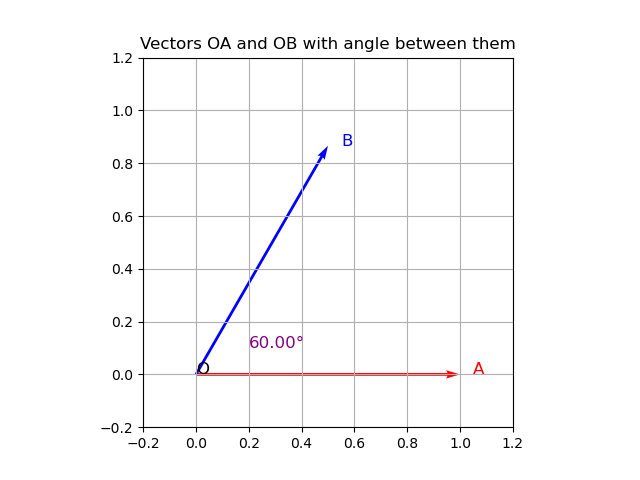
\includegraphics[width=0.8\linewidth]{figs/Figure_1.png}
    \label{fig:placeholder}
\end{figure}
\end{document}